\begin{figure*}[t]
\centering
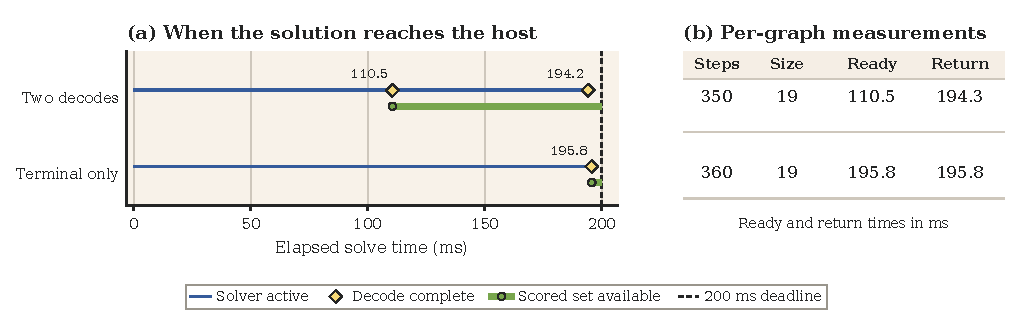
\includegraphics[width=\textwidth]{figures/solve_clock.pdf}
\caption{\textbf{Two decoding schedules on the same RB graph} (242 vertices, seed 1017). (a) Timing starts with per-graph buffer loading and particle reset. The blue line ends when the solver returns. Diamonds mark completed decodes. The green segment starts when the ultimately scored set reaches the host and extends to the 200~ms deadline. The midpoint decode yields 19 vertices at 110.5~ms, and the terminal decode at 194.2~ms ties that size. With only a terminal decode, 19 vertices become available at 195.8~ms. (b) The two runs reach the same size in 350 and 360 steps, respectively.}
\label{fig:solve-clock}
\end{figure*}
